\documentclass{article}
\usepackage[UTF8]{ctex}

\usepackage{amsmath}        %数学公式
\usepackage{amssymb}
\usepackage{cases}          %联立编号
\usepackage{cite}           %引用

\usepackage{graphicx}       %插入图片
\usepackage{float}          %设置图片浮动位置
\usepackage{subfigure}      %插入多图时用子图显示

\usepackage{listings}
\usepackage{xcolor}

\usepackage{anyfontsize}    %解决一个奇怪的字体大小报错问题
\usepackage{fancyhdr}       %页眉、页脚、页码
\usepackage[a4paper, margin=1in]{geometry}    %纸张大小
\usepackage{longtable}

\lstset{
    basicstyle          =   \sffamily,          % 基本代码风格
    keywordstyle        =   \bfseries,          % 关键字风格
    commentstyle        =   \rmfamily\itshape,  % 注释的风格,斜体
    stringstyle         =   \ttfamily,  % 字符串风格
    flexiblecolumns,                % 别问为什么,加上这个
    numbers             =   left,   % 行号的位置在左边
    showspaces          =   false,  % 是否显示空格,显示了有点乱,所以不现实了
    numberstyle         =   \zihao{-5}\ttfamily,    % 行号的样式,小五号,tt等宽字体
    showstringspaces    =   false,
    captionpos          =   t,      % 这段代码的名字所呈现的位置,t指的是top上面
    frame               =   lrtb,   % 显示边框
}

\lstdefinestyle{Python}{
    language        =   Python, % 语言选Python
    basicstyle      =   \zihao{-5}\ttfamily,
    numberstyle     =   \zihao{-5}\ttfamily,
    keywordstyle    =   \color{blue},
    keywordstyle    =   [2] \color{teal},
    stringstyle     =   \color{magenta},
    commentstyle    =   \color{red}\ttfamily,
    breaklines      =   true,   % 自动换行,建议不要写太长的行
    columns         =   fixed,  % 如果不加这一句,字间距就不固定,很丑,必须加
    basewidth       =   0.5em,
}

\newcommand\f[2]{\frac{#1}{#2}}
\newcommand\pf[2]{\frac{\partial#1}{\partial#2}}
\newcommand\df[2]{\dfrac{#1}{#2}}
\newcommand\pdf[2]{\dfrac{\partial#1}{\partial#2}}
\newcommand\po[2]{\frac{e^{-#2}#2^#1}{#1!}}

\title{\bf\huge 概率论与数理统计 - 作业 5}
\author{Jerry}
\date{\today}

\begin{document}
\maketitle

\section*{T1. }

\subsubsection*{(1.)}

随机向量$(X,Y)$的分布表是:

\begin{table}[H]
    \centering
    \begin{tabular}{|l|l|l|l|l|}
        \hline
        $X$ \textbackslash $Y$ & ~~$0$~~ & ~~$1$~~ & ~~$2$~~ & ~~$3$~~ \\ \hline
        $~~~0$ & ~~$\f{1}{22}$ & ~~$\f{2}{11}$ & ~~$\f{3}{22}$ & ~~$\f{1}{55}$ \\ \hline
        $~~~1$ & ~~$\f{3}{22}$ & ~~$\f{3}{11}$ & ~~$\f{9}{110}$ & ~~$0$ \\ \hline
        $~~~2$ & ~~$\f{3}{44}$ & ~~$\f{3}{55}$ & ~~$0$ & ~~$0$ \\ \hline
        $~~~3$ & ~~$\f{1}{220}$ & ~~$0$ & ~~$0$ & ~~$0$ \\ \hline
    \end{tabular}
\end{table}

\subsubsection*{(2.)}

$P(X=1)=\f{3}{22}+\f{3}{11}+\f{9}{110}=\f{27}{55}$

\section*{T2. }

\begin{equation}
    \begin{aligned}
        P(a < X \leq b, c < Y \leq d)
        & = P(x \leq b, c < y \leq d)-P(x \leq a, c < y \leq d)\\
        & = P(x \leq b, y \leq d)-P(x \leq b, y \leq c)-P(x \leq a, y \leq d)+P(x \leq a, y \leq c)\\
        & = F(b,d)-F(b,c)-F(a,d)+F(a,c)
    \end{aligned}
\end{equation}

\section*{T3. }

\subsubsection*{(1.)}

\[
    f(X,Y)=
    \begin{cases}
        \f{1}{x^2+y^2}, &\quad x^2+y^2\leq1\\
        0, &\quad \text{其他}
    \end{cases}
\]

\subsubsection*{(2.)}

$X$的边际分布函数的概率密度函数$f_X(x)=\int_{-\sqrt{1-x^2}}^{\sqrt{1-x^2}}\f{1}{x^2+y^2}dy=\f{1}{x}\arctan(\f{y}{x})|_{-\sqrt{1-x^2}}^{\sqrt{1-x^2}}=\f{1}{x}\arctan(\f{\sqrt{1-x^2}}{x})-\f{1}{x}\arctan(\f{-\sqrt{1-x^2}}{x})=\f{2}{x}\arctan(\f{\sqrt{1-x^2}}{x})$

$Y$的边际分布函数的概率密度函数$f_Y(y)=\int_{-\sqrt{1-y^2}}^{\sqrt{1-y^2}}\f{1}{x^2+y^2}dx=\f{1}{y}\arctan(\f{x}{y})|_{-\sqrt{1-y^2}}^{\sqrt{1-y^2}}=\f{1}{y}\arctan(\f{\sqrt{1-y^2}}{y})-\f{1}{y}\arctan(\f{-\sqrt{1-y^2}}{y})=\f{2}{y}\arctan(\f{\sqrt{1-y^2}}{y})$

\subsubsection*{(3.)}

$P(R \leq r)=\f{\pi 1^2 -\pi r^2}{\pi 1^2}=1-r^2$

\subsubsection*{(4.)}

$E(R)=\int_0^1P(R)dR=\int_0^1(1-R^2)dR=\f{2}{3}$

\section*{T4. }

二元正态分布:$f(x,y)=\f{1}{2\pi\sigma_1\sigma_2\sqrt{1-\rho^2}}\exp\{-\f{1}{2(1-\rho^2)}[\f{(x-\mu_1)^2}{\sigma_1^2}-2\rho\f{(x-\mu_1)(y-\mu_2)}{\sigma_1\sigma_2}+\f{(y-\mu_2)^2}{\sigma_2^2}]\}$

计算二元正态分布的边际密度函数:

\begin{equation}
    \begin{aligned}
        f_X(x)
        & = \int_{-\infty}^{\infty}\f{1}{2\pi\sigma_1\sigma_2\sqrt{1-\rho^2}}\exp\{-\f{1}{2(1-\rho^2)}[\f{(x-\mu_1)^2}{\sigma_1^2}-2\rho\f{(x-\mu_1)(y-\mu_2)}{\sigma_1\sigma_2}+\f{(y-\mu_2)^2}{\sigma_2^2}]\}dy\\
        & = \f{1}{2\pi\sigma_1\sigma_2\sqrt{1-\rho^2}}[\int_{-\infty}^{\infty}\exp\{-\f{1}{2(1-\rho^2)}[\f{(x-\mu_1)^2}{\sigma_1^2}-2\rho\f{(x-\mu_1)(y-\mu_2)}{\sigma_1\sigma_2}+\f{(y-\mu_2)^2}{\sigma_2^2}]\}dy]\\
        & = \f{1}{2\pi\sigma_1\sigma_2\sqrt{1-\rho^2}}\exp\{-\f{1}{2(1-\rho^2)}\f{(x-\mu_1)^2}{\sigma_1^2}\}[\int_{-\infty}^{\infty}\exp\{-\f{1}{2(1-\rho^2)}[-2\rho\f{(x-\mu_1)(y-\mu_2)}{\sigma_1\sigma_2}+\f{(y-\mu_2)^2}{\sigma_2^2}]\}dy]\\
        & = \f{1}{\sqrt{2\pi}\sigma_1}\exp\{-\f{(x-\mu_1)^2}{2\sigma_1^2}\}[\int_{-\infty}^{\infty}\f{1}{\sqrt{2\pi}\sigma_2\sqrt{1-\rho^2}}\exp\{-\f{1}{2(1-\rho^2)}[-2\rho\f{(x-\mu_1)(y-\mu_2)}{\sigma_1\sigma_2}+\f{(y-\mu_2)^2}{\sigma_2^2}]\}dy]\\
        & = \f{1}{\sqrt{2\pi}\sigma_1}\exp\{-\f{(x-\mu_1)^2}{2\sigma_1^2}\}
    \end{aligned}
\end{equation}

同理,$f_Y(y)=\f{1}{\sqrt{2\pi}\sigma_2}\exp\{-\f{(y-\mu_2)^2}{2\sigma_2^2}\}$

\section*{T5. }

计算二元正态分布的条件密度函数:

$f(x|y) = \f{f(x,y)}{f_Y(y)} = \f{1}{\sqrt{2\pi}\sigma_1\sqrt{1-\rho^2}}\exp\{-\f{[x-(\mu_1+\rho\f{\sigma_1}{\sigma_2}(y-\mu_2))]^2}{2\sigma_1^2(1-\rho^2)}\}$

同理,$f(y|x)=\f{1}{\sqrt{2\pi}\sigma_2\sqrt{1-\rho^2}}\exp\{-\f{[y-(\mu_2+\rho\f{\sigma_2}{\sigma_1}(x-\mu_1))]^2}{2\sigma_2^2(1-\rho^2)}\}$

\section*{T6. }

\subsubsection*{(1.)}

$
    f(x,y)=
    \begin{cases}
        2, &\quad 0<y<1,0<x<y\\
        0, &\quad \text{其他}
    \end{cases}
$

\subsubsection*{(2.)}

$f_Y(y)=\int_{-\infty}^{\infty}f(x,y)dx=\int_{0}^{y}2dx=2y$

\subsubsection*{(3.)}

$
    f(x|y)=\f{f(x,y)}{f_Y(y)}=\f{f(x,y)}{2}=
    \begin{cases}
        y, &\quad 0<y<1,0<x<y\\
        0, &\quad \text{其他}
    \end{cases}
$

\section*{T7. }

$X_1\sim P(\lambda_1)$,$X_2\sim P(\lambda_2)$

$F(x_1)=1-e^{-\lambda_1x_1}$,$F(x_2)=1-e^{-\lambda_2x_2}$

$f(x_1)=\lambda_1e^{-\lambda_1x_1}$,$f(x_2)=\lambda_2e^{-\lambda_2x_2}$

\subsubsection*{(1.)}

$X_1+X_2=n$

\begin{equation}
    \begin{aligned}
        P(X_1=k|X_1+X_2=n)
        & = \f{P(X_1=k,X_1+X_2=n)}{P(X_1+X_2=n)}\\
        & = \f{P(X_1=k,X_2=n-k)}{P(X_1+X_2=n)}\\
        & = \f{P(X_1=k)P(X_2=n-k)}{P(X_1+X_2=n)}\\
        & = \f{e^{-\lambda_1k}\cdot\f{\lambda_1^k}{k!}\cdot e^{-\lambda_2(n-k)}\cdot\f{\lambda_2^{n-k}}{(n-k)!}}{e^{-(\lambda_1+\lambda_2)n}\cdot\f{(\lambda_1+\lambda_2)^n}{n!}}\\
        & = \f{n!}{k!(n-k)!}\cdot\f{\lambda_1^k\lambda_2^{n-k}}{(\lambda_1+\lambda_2)^n}\cdot e^{\lambda_1(n-k)+\lambda_2k}\\
    \end{aligned}
\end{equation}

\subsubsection*{(2.)}

$P(X_1=k|X_1+X_2=n)=C_n^k\cdot\f{\lambda_1^k\lambda_2^{n-k}}{(\lambda_1+\lambda_2)^n}\cdot e^{\lambda_1(n-k)+\lambda_2k}$

可以看做$n$中取$k$的组合数,每种组合的概率为$\f{\lambda_1^k\lambda_2^{n-k}}{(\lambda_1+\lambda_2)^n}\cdot e^{\lambda_1(n-k)+\lambda_2k}$

\section*{T8. }

\subsubsection*{(1.)}

假设甲到达的时间为$X$,乙到达的时间为$Y$,则$X\sim U(0,60)$,$Y\sim U(0,60)$(取分钟为单位)

$f(x,y)=
\begin{cases}
    \f{1}{3600}, &\quad 0<x<60,0<y<60\\
    0, &\quad \text{其他}
\end{cases}
$

\subsubsection*{(2.)}

先到的人等待10分钟的概率为$P(X>Y+10)+P(Y>X+10)$

\begin{equation}
    \begin{aligned}
        P(X>Y+10)+P(Y>X+10)
        & = \int_{0}^{50}\int_{y+10}^{60}\f{1}{3600}dxdy+\int_{0}^{50}\int_{x+10}^{60}\f{1}{3600}dydx\\
        & = \int_{0}^{50}\f{1}{3600}\int_{y+10}^{60}dxdy+\int_{0}^{50}\f{1}{3600}\int_{x+10}^{60}dydx\\
        & = \int_{0}^{50}\f{1}{3600}(60-y-10)dy+\int_{0}^{50}\f{1}{3600}(60-x-10)dx\\
        & = \int_{0}^{50}\f{1}{3600}(50-y)dy+\int_{0}^{50}\f{1}{3600}(50-x)dx\\
        & = \f{1}{3600}(50y-\f{y^2}{2})|_0^{50}+\f{1}{3600}(50x-\f{x^2}{2})|_0^{50}\\
        & = \f{1}{3600}(2500-\f{2500}{2})+\f{1}{3600}(2500-\f{2500}{2})\\
        & = \f{25}{36}\\
    \end{aligned}
\end{equation}

\section*{T9. }

$\forall \alpha \in [-1,1]$,$$H(x,y)=F(x)G(y)\{1+\alpha[1-F(x)][1-G(y)]\}$$

\subsubsection*{(1.)}

$F_Y(x)=\lim_{y\to\infty}H(x,y)=F(x)$

$G_X(y)=\lim_{x\to\infty}H(x,y)=G(y)$

\subsubsection*{(2.)}

构造$F(x)=x$,$G(y)=y$,则$H(x,y)=xy\{1+\alpha[1-x][1-y]\}$

此时边际分布都是[0,1]上的均匀分布,分别取$\alpha=-1,1$即可构造出两个不同的二元分布

\section*{T10. }

$H(x,y)=F(x)G(y)\{1+\alpha[1-F(x)][1-G(y)]\}$即可

\section*{T11. }

\subsubsection*{(1.)$X$离散,$Y$离散}

全概率公式:$f_X(x)=f_X(x)=\sum_{i=1}^{\infty}f(x,y_i)=\sum_{i=1}^{\infty}f(x|y_i)f_Y(y_i)$

$Bayes$公式:$f_{Y|X}(y|x)=\f{f(x|y)f_Y(y)}{f_X(x)}=\f{f(x|y)f_Y(y)}{\sum_{i=1}^{\infty}f(x|y_i)f_Y(y_i)}$

\subsubsection*{(2.)$X$离散,$Y$连续}

全概率公式:$f_X(x)=\int_{-\infty}^{\infty}f(x,y)dy=\int_{-\infty}^{\infty}f(x|y)f_Y(y)dy$

$Bayes$公式:$f_{Y|X}(y|x)=\f{f(x|y)f_Y(y)}{f_X(x)}=\f{f(x|y)f_Y(y)}{\int_{-\infty}^{\infty}f(x|y)f_Y(y)dy}$

\subsubsection*{(3.)$X$连续,$Y$离散}

全概率公式:$f_X(x)=f_X(x)=\sum_{i=1}^{\infty}f(x,y_i)=\sum_{i=1}^{\infty}f(x|y_i)f_Y(y_i)$

$Bayes$公式:$f_{Y|X}(y|x)=\f{f(x|y)f_Y(y)}{f_X(x)}=\f{f(x|y)f_Y(y)}{\sum_{i=1}^{\infty}f(x|y_i)f_Y(y_i)}$

\subsubsection*{(4.)$X$连续,$Y$连续}

全概率公式:$f_X(x)=\int_{-\infty}^{\infty}f(x,y)dy=\int_{-\infty}^{\infty}f(x|y)f_Y(y)dy$

$Bayes$公式:$f_{Y|X}(y|x)=\f{f(x|y)f_Y(y)}{f_X(x)}=\f{f(x|y)f_Y(y)}{\int_{-\infty}^{\infty}f(x|y)f_Y(y)dy}$

\section*{T12. }

$$f(x,y)=
\begin{cases}
    \f{c}{1+x^2+y^2}, &\quad x^2+y^2\leq1\\
    0, &\quad x^2+y^2>1
\end{cases}
$$

\subsubsection*{(1.)}

\begin{equation}
    \begin{aligned}
        \int_{-\infty}^{\infty}\int_{-\infty}^{\infty}f(x,y)dxdy
        & =\int_{-\infty}^{\infty}\int_{-\infty}^{\infty}\f{c}{1+x^2+y^2}dxdy\\
        & =\int_{0}^{2\pi}\int_{0}^{1}\f{c}{1+r^2}rdrd\theta\\
        & =\int_{0}^{2\pi}d\theta\int_{0}^{1}\f{c}{1+r^2}rdr\\
        & =2\pi c\int_{0}^{1}\f{r}{1+r^2}dr\\
        % & =2\pi c[\f{1}{2}\ln(1+r^2)]|_0^1\\
        & =\pi c\ln2=1\\
    \end{aligned}
\end{equation}

故$c=\f{1}{\pi\ln2}$

\subsubsection*{(2.)}

$f(x,y)=
\begin{cases}
    \df{1}{\pi\ln2(1+x^2+y^2)}, &\quad x^2+y^2\leq1\\
    0, &\quad x^2+y^2>1
\end{cases}
$

\begin{equation}
    \begin{aligned}
        f_Y(x)=
        & =\int_{-\infty}^{\infty}\f{1}{\pi\ln2(1+x^2+y^2)}dy\\
        & =\f{1}{\pi\ln2}\int_{-\infty}^{\infty}\f{1}{1+x^2+y^2}dy\\
        & =\f{1}{\pi\ln2}\int_{0}^{2\pi}\int_{0}^{1}\f{1}{1+r^2}rdrd\theta\\
        & =\f{1}{\pi\ln2}\int_{0}^{2\pi}d\theta\int_{0}^{1}\f{1}{1+r^2}rdr\\
        & =\f{1}{\pi\ln2}\cdot2\pi\cdot\f{1}{2}\ln2\\
        & =\f{1}{\pi\ln2}\ln2\\
        & =\f{1}{\pi}\\
    \end{aligned}
\end{equation}

同理,$f_X(y)=\f{1}{\pi}$

$f(x,y)\neq f(x)\cdot f(y)$,故$X,Y$不独立

\section*{T13. }

$X \sim N(0,1)$,$Y \sim N(0,1)$

\subsubsection*{(1.)}

$$g(x,y)=
\begin{cases}
    f(x,y)+\df{xy}{100}, &\quad x^2+y^2\leq1\\
    f(x,y), &\quad x^2+y^2>1
\end{cases}
$$

$\int_{-\infty}^{\infty}\int_{-\infty}^{\infty}g(x,y)dxdy=\int_{-\infty}^{\infty}\int_{-\infty}^{\infty}f(x,y)dxdy+\int_{-\infty}^{\infty}\int_{-\infty}^{\infty}\df{xy}{100}dxdy=1+0=1$,得证

\subsubsection*{(2.)}

$(U,V)$密度函数是$g(x,y)$

$G_V(U)=\int_{-\infty}^{\infty}g(x,y)dy=\int_{-\infty}^{\infty}f(x,y)dy+\int_{-\infty}^{\infty}\df{xy}{100}dy=F_X(x)+0=F_X(x)$

同理,$G_U(V)=F_Y(y)$

故$U,V$都服从正态分布

证明$(U,V)$的联合密度函数不符合二元正态分布的形式:

$g(u,v)\neq f(u)\cdot f(v)$,故$U,V$不独立,故不服从二元正态分布

\section*{T14. }

\begin{center}
    \begin{figure}[H] %H为当前位置,!htb为忽略美学标准,htbp为浮动图形
        \centering %图片居中
        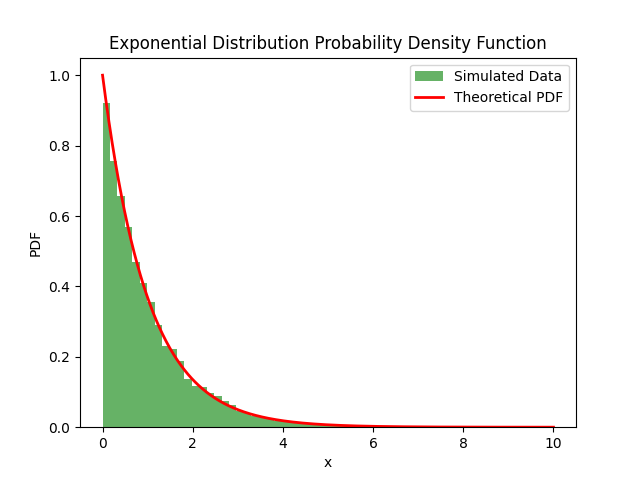
\includegraphics[width=0.8\textwidth]{img/Figure_1.png} %插入图片,[]中设置图片大小,{}中是图片文件名
        \caption{直方图\&概率密度函数图} %最终文档中希望显示的图片标题
        \label{fig1} %用于文内引用的标签
    \end{figure}
\end{center}

\subsubsection*{Code}

源代码如下:

\lstinputlisting[
    style       =   Python,
    caption     =   {\bf simulation1.py},
    label       =   {1}
]{code/simulation1.py}

\end{document}
